\documentclass[11pt,a4paper]{article}
\usepackage[margin=2.2cm]{geometry}
\usepackage[T1]{fontenc}
\usepackage{lmodern}
\usepackage{graphicx}
\usepackage{booktabs}
\usepackage{float}
\usepackage[section]{placeins}
\usepackage{titlesec}
\newcommand{\sectionbreak}{\clearpage}
\setcounter{tocdepth}{1}
\usepackage{caption}
\usepackage{subcaption}
\usepackage{enumitem}
\usepackage{xcolor}
\usepackage{amsmath}
\usepackage{array}
\usepackage[hidelinks]{hyperref}
\emergencystretch=3em
\setlength{\textfloatsep}{14pt plus 2pt minus 2pt}
\setlength{\floatsep}{12pt plus 2pt minus 2pt}
\setlength{\intextsep}{12pt plus 2pt minus 2pt}
\renewcommand{\topfraction}{0.9}
\renewcommand{\bottomfraction}{0.8}
\renewcommand{\textfraction}{0.1}
\renewcommand{\floatpagefraction}{0.75}
\makeatletter
\setlength{\@fptop}{0pt}
\setlength{\@fpsep}{14pt}
\setlength{\@fpbot}{0pt plus 1fil}
\makeatother

\graphicspath{{figs/}}
\setlist{itemsep=2pt, topsep=4pt}
\captionsetup{font=small, labelfont=bf}
\newcommand{\ft}[1]{\texttt{#1}}


\title{\textbf{Formula 1 Podium Prediction}\\[4pt]\large Milestone 1 --- Analytical Report}
\author{Team: \textit{[add team member names and IDs]}}
\date{October 2026}

\begin{document}
\maketitle

\begin{abstract}
We predict whether a driver will finish on the podium (\ft{positionOrder} $\leq 3$) using only information available after qualifying and before the race starts. We clean and audit the 14 relational Ergast tables (1950--2024) and build a leakage-safe modeling table with exactly one row per driver per race (26,668 rows, 12.7\% podiums). We answer three data-engineering questions with multi-hop joins, then train a logistic-regression baseline, a random forest and a shallow neural network on a chronological split. On the unseen 2022--2024 test set all three models reach ROC-AUC $\approx$ 0.92--0.93 and PR-AUC $\approx$ 0.65--0.67. The random forest has the best PR-AUC, our primary metric. Ablation and explainability (permutation importance, SHAP, LIME) show that every model is anchored on starting position, with championship form as the second signal. These explanations describe what the models rely on, \emph{not} what causes podium finishes.
\end{abstract}

\tableofcontents

%=====================================================================
\section{Task, Data and Prediction Cutoff}
\begin{itemize}
  \item \textbf{Data:} Formula 1 World Championship 1950--2024 (Kaggle/Ergast), 14 linked CSV tables.
  \item \textbf{Unit of analysis:} one driver entering one race, i.e.\ the key (\ft{raceId}, \ft{driverId}) must be unique.
  \item \textbf{Target:} \ft{target\_podium} $= 1$ if \ft{positionOrder} $\leq 3$, else 0.
  \item \textbf{Prediction cutoff:} after qualifying, before the race starts. Current-race results, status, points, laps, pit stops, lap times and post-race standings are excluded as features. Pit stops, lap times and race status are used only for auditing and to answer the data-engineering questions.
\end{itemize}

%=====================================================================
\section{Data Audit and Cleaning}

\subsection{Sentinel audit (before cleaning)}
The raw CSVs encode missing values as the literal string \verb|\N|. All tables were loaded as strings, so no sentinel was silently converted. The audit found missing values or sentinels in 6 of the 14 tables (Figure~\ref{fig:sentinel}). The missingness has three different origins:
\begin{itemize}
  \item \textbf{Post-race fields} (\ft{results}: \ft{time}/\ft{milliseconds} 71.3\%, \ft{fastestLap*} 69.2\%, \ft{position} 40.9\%). These are leakage and are never used as features.
  \item \textbf{Structural qualifying gaps} (\ft{q2} 44.1\%, \ft{q3} 65.0\%). These are caused by changes in the qualifying format and are analysed in Section~\ref{sec:quali}.
  \item \textbf{Fields recorded only recently or rarely} (session dates in \ft{races} $>$92\%; driver \ft{number}/\ft{code}). These were dropped or kept as metadata only.
\end{itemize}
All cleaning works on copies; the raw tables are never modified.

\begin{figure}[!htbp]
  \centering
  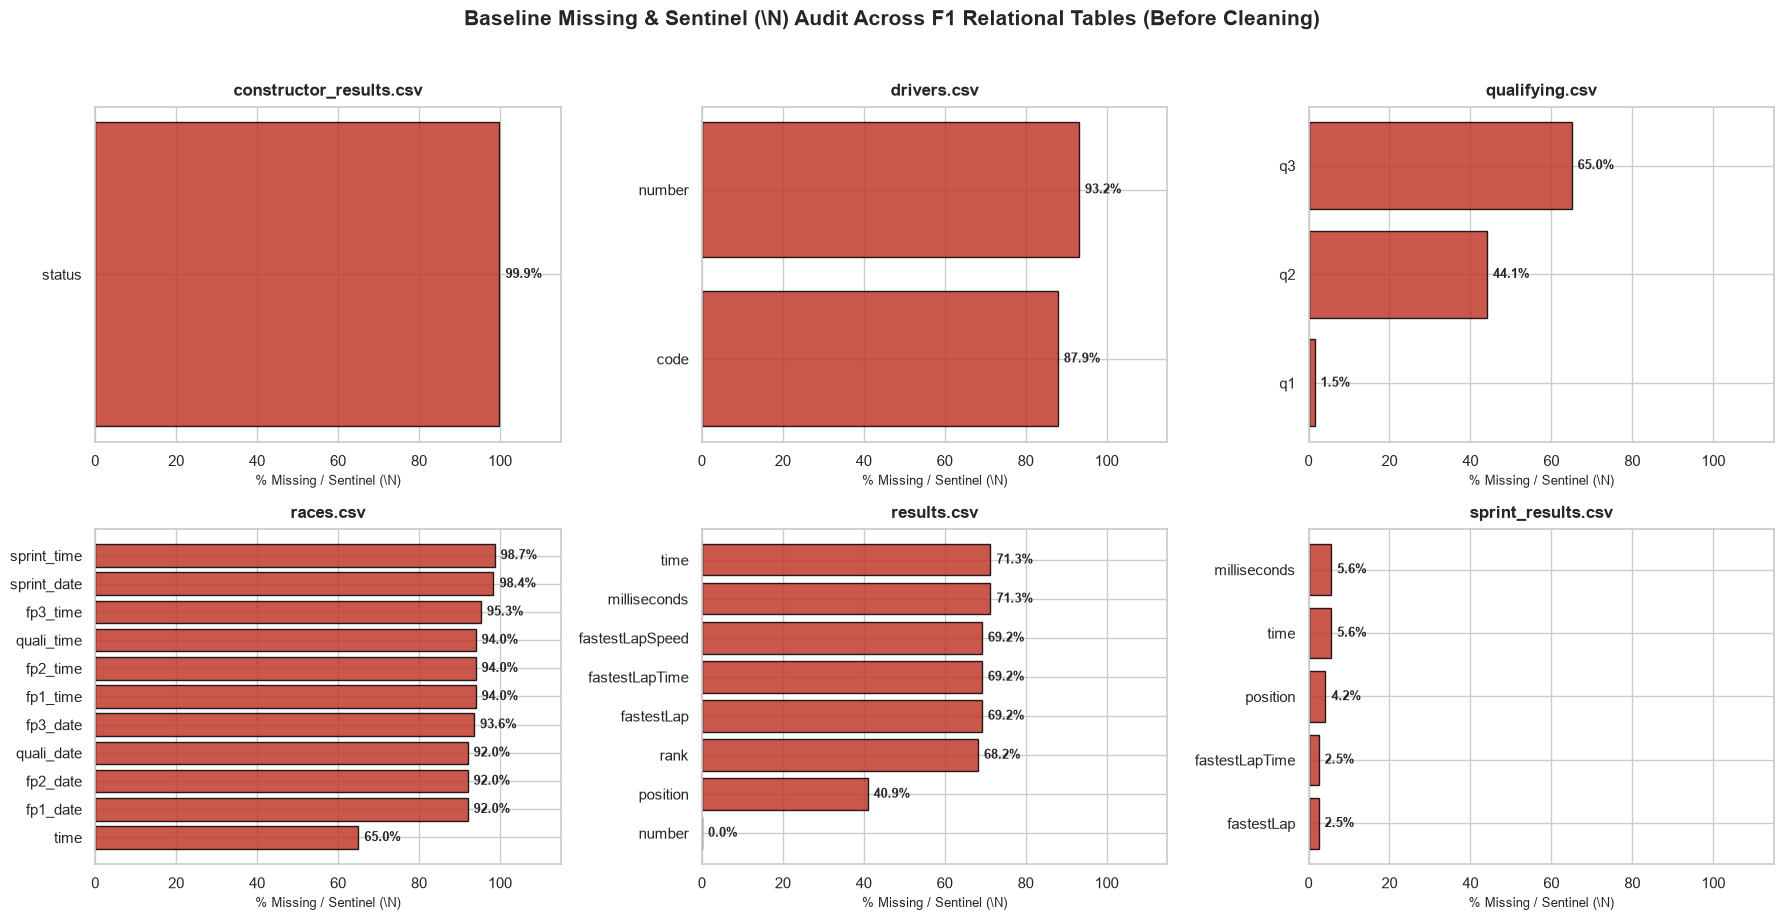
\includegraphics[width=\textwidth]{c04_1.png}
  \caption{Missing and sentinel (\texttt{\textbackslash N}) values per column, before cleaning.}
  \label{fig:sentinel}
\end{figure}

\subsection{Sentinels and semantic typing}
\begin{itemize}
  \item \verb|\N| is replaced by \ft{NaN} in every table. A hidden sentinel, \ft{rank} $= 0$ (``no fastest lap''), is also neutralised to \ft{NaN}.
  \item \textbf{Dates:} \ft{dob}, race dates and session dates are parsed to \ft{datetime}.
  \item \textbf{Durations:} qualifying lap strings (\ft{m:ss.mmm}) are converted to seconds (\ft{q1\_sec}, \ft{q2\_sec}, \ft{q3\_sec}). Pit-stop durations come from \ft{milliseconds}/1000, because the raw string mixes two formats.
  \item \textbf{Constructor results:} \ft{status} (\ft{D} or \verb|\N|) becomes a boolean \ft{constructor\_disqualified}.
  \item \textbf{Race status:} all 139 status strings are mapped to functional groups (\ft{mechanical}, \ft{accident\_collision}, \ft{driver\_team\_error}, \ft{regulation}, \ft{did\_not\_start}, \ft{finished}, \ft{lapped\_finish}, \ldots). This mapping is used for the duplicate rule and for Question~3.
\end{itemize}

\subsection{Qualifying coverage and the pace feature}\label{sec:quali}
Each driver's best qualifying lap is normalised to the pole time of the same race:
\[ \text{gap\_to\_pole\_pct} = \left(\frac{\text{best lap}}{\text{pole lap}} - 1\right)\times 100. \]
This makes pace comparable across circuits of different length and across wet and dry sessions. The missing qualifying values are not random (Figures~\ref{fig:qmiss}--\ref{fig:qelim}):
\begin{itemize}
  \item \textbf{1994--2005:} single-session qualifying, so \ft{q2}/\ft{q3} are 100\% missing by design.
  \item \textbf{From 2006 (knockout format):} Q2 is missing for about 25--30\% of drivers and Q3 for about 50\%. In this era a missing value means the driver was eliminated in an earlier session.
\end{itemize}
Rows are therefore \emph{not} dropped, since that would keep only the fastest cars of the modern era (survivor bias). For the outlier rule, laps more than 100\% slower than pole would be set to \ft{NaN}; zero laps exceeded this threshold (Figure~\ref{fig:qout}). The rule deliberately avoids a 3-standard-deviation cut, which would delete legitimate wet-session laps.

\begin{figure}[!htbp]
  \centering
  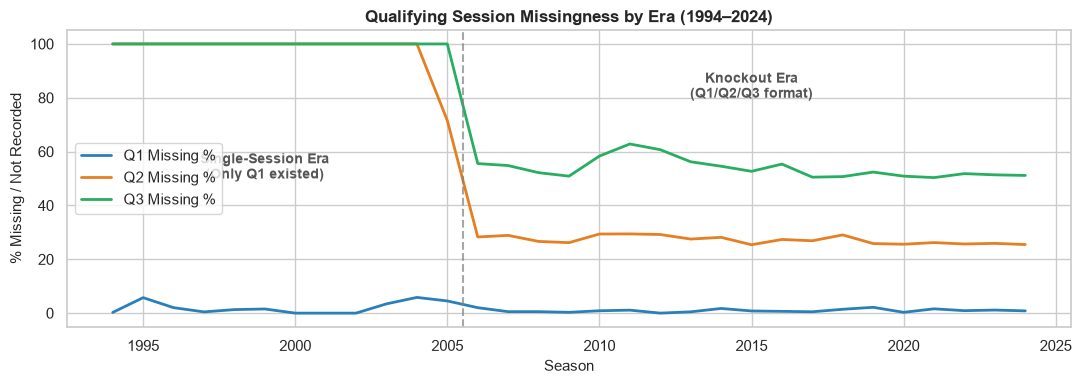
\includegraphics[width=0.85\textwidth]{c14_1.png}
  \caption{Qualifying-session missingness by season. The single-session era (1994--2005) has no Q2/Q3 by design.}
  \label{fig:qmiss}
\end{figure}

\begin{figure}[!htbp]
  \centering
  \begin{subfigure}{0.49\textwidth}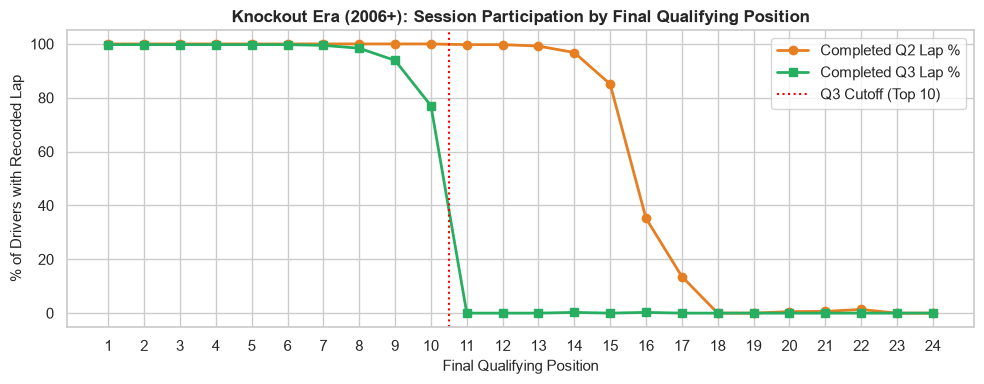
\includegraphics[width=\textwidth]{c16_1.png}\caption{Knockout era: session coverage by position. Missing means eliminated.}\label{fig:qelim}\end{subfigure}
  \hfill
  \begin{subfigure}{0.49\textwidth}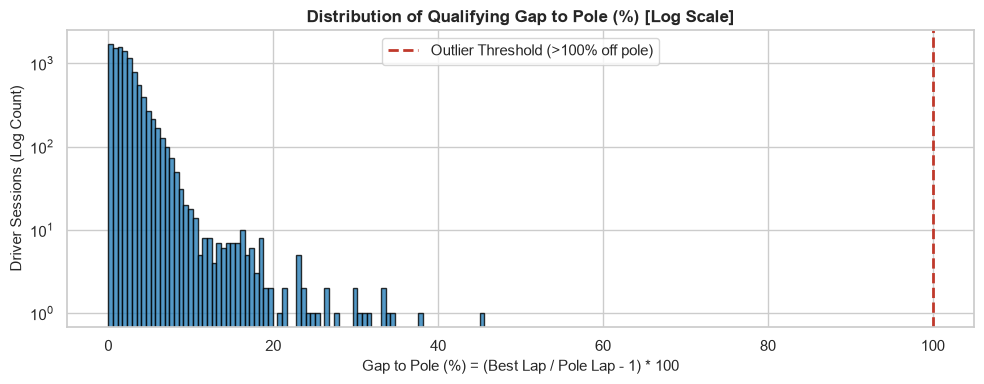
\includegraphics[width=\textwidth]{c18_1.png}\caption{Log-scale \ft{gap\_to\_pole\_pct}; no lap exceeds the 100\% threshold.}\label{fig:qout}\end{subfigure}
  \caption{Evidence for how missing qualifying data and outliers are handled.}
\end{figure}

\subsection{Primary and foreign keys}
Primary keys of \ft{drivers}, \ft{constructors}, \ft{circuits}, \ft{races}, \ft{results}, \ft{status}, \ft{qualifying} and \ft{constructor\_results} are all unique and non-null. All eight checked foreign-key relationships reconcile with zero orphans:
\begin{itemize}
  \item \ft{results} $\to$ \ft{races}, \ft{drivers}, \ft{constructors} and \ft{status};
  \item \ft{qualifying} $\to$ \ft{races} and \ft{drivers};
  \item \ft{constructor\_results} $\to$ \ft{races} and \ft{constructors}.
\end{itemize}

\subsection{Grain: one row per (raceId, driverId)}
\ft{results} contains 176 rows involved in duplicated (\ft{raceId}, \ft{driverId}) pairs, i.e.\ 91 excess rows. They all come from \textbf{shared drives}, where a driver took over another car mid-race. These occur mostly in 1950--1964, plus one case in 1978 (Figure~\ref{fig:dups}). We keep one row per pair using a deterministic three-tier rule:
\begin{enumerate}
  \item prefer the entry that was \textbf{classified} (finished or lapped finish) over a retired entry;
  \item then the better \textbf{finishing position} (lowest \ft{positionOrder});
  \item then the entry with more \textbf{laps} completed.
\end{enumerate}
\textbf{Why:} the target asks whether the driver reached the podium in that race. Keeping a retired chassis over the car the driver brought home would record a false ``no podium''. As Figure~\ref{fig:dups} (right) shows, the dropped rows are mostly mechanical retirements and accidents. The resulting table has \textbf{26,668 rows} (from 26,759), the key is verified unique and non-null, and 3,395 rows (12.7\%) are podiums.

\begin{figure}[!htbp]
  \centering
  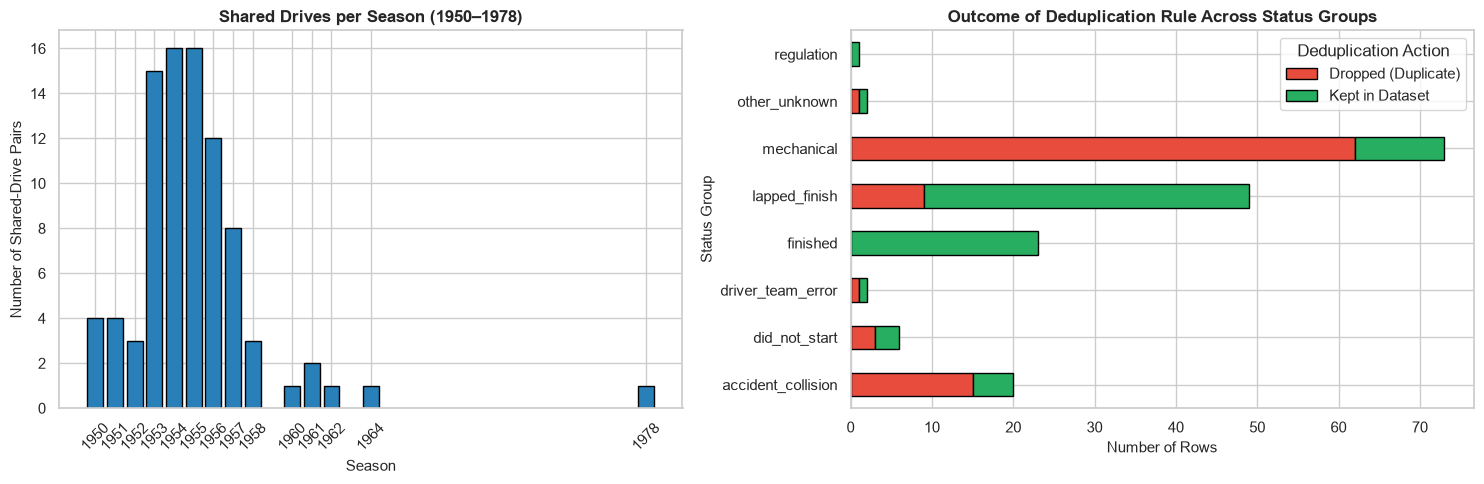
\includegraphics[width=\textwidth]{c25_1.png}
  \caption{Left: shared-drive duplicates per season. Right: status of the rows kept and dropped by the duplicate rule.}
  \label{fig:dups}
\end{figure}

%=====================================================================
\section{Data-Engineering Questions}

\subsection{Q1. Which circuits convert a front-row start into a podium most often, and does the ranking change after 2014?}
\textbf{Method and joins.} \ft{results} (grid, outcome) $\bowtie$ \ft{races} (year, Grand Prix) $\bowtie$ \ft{qualifying} (qualifying position). The conversion rate is podiums divided by front-row starts, computed per Grand Prix and era: pre-2014 vs.\ the 2014+ hybrid era. Only Grands Prix with at least 10 front-row starts in \emph{both} eras are compared (17 events).

\textbf{Grid vs.\ qualifying.} A front-row start is defined by \ft{grid} $\in\{1,2\}$, the actual starting slot after penalties, not by qualifying position. The two differ: in 36 front-row starts the driver had qualified 3rd or lower and was promoted by penalties to cars ahead.

\textbf{Answer.} In the hybrid era the \textbf{Japanese GP (88.9\%)}, \textbf{Abu Dhabi GP (86.4\%)} and \textbf{Monaco GP (85.0\%)} convert front-row starts most often (Figure~\ref{fig:q1}). The ranking \textbf{does change substantially}:
\begin{itemize}
  \item The rank correlation between the two eras is essentially zero (Spearman $\rho = 0.02$, $p = 0.94$).
  \item Monaco moves from 16th to 3rd, and the Hungarian GP falls from 2nd (67.9\%) to last (59.1\%). Japan is the only Grand Prix ranked 1st in both eras.
  \item Conversion rose at 16 of the 17 Grands Prix, from a mean of 57.1\% to 76.7\% (Wilcoxon signed-rank $p < 0.001$). Front-row starts became much more reliable overall in the hybrid era.
\end{itemize}

\textbf{Grain, missing data and cutoff.} The grain is one row per driver per race, restricted to the two front-row starters. \ft{grid} comes from \ft{results} and is complete, so the gaps in the qualifying table (pre-1994 and single-session years) do not affect the rates. Qualifying position is used only to show the difference between grid and qualifying. Both \ft{grid} and qualifying are known before the race starts.

\textbf{Caveat.} Hybrid-era rates rest on at most 22 front-row starts per Grand Prix (two per race, 2014--2024), so neighbouring ranks are within sampling noise. Grands Prix are grouped by event name, which can span more than one circuit layout over the decades.

\begin{figure}[!htbp]
  \centering
  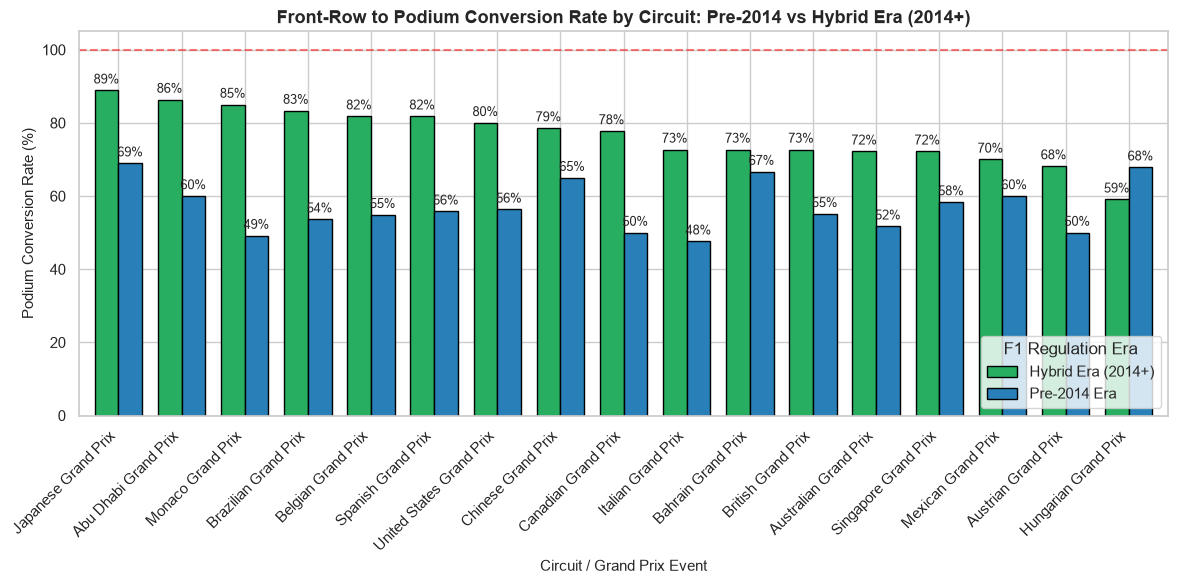
\includegraphics[width=\textwidth]{c34_1.png}
  \caption{Front-row-to-podium conversion rate per Grand Prix, pre-2014 vs.\ hybrid era (2014+), sorted by hybrid-era rate.}
  \label{fig:q1}
\end{figure}

\subsection{Q2. Do drivers podium more often at home, after controlling for starting position?}
\textbf{Method and joins.} \ft{drivers} (nationality mapped to a country) $\bowtie$ \ft{races} $\bowtie$ \ft{circuits} (country) gives the flag \ft{is\_home\_race}, which is then joined with \ft{results} for the outcome. To control for starting position, podium rates are compared \emph{within} grid tiers: front row (P1--2), rows 2--3 (P3--6), midfield (P7--12) and backmarkers (P13+). Pit-lane and non-standard starts (\ft{grid} $=0$) are excluded.

\textbf{Answer: no.} Within every grid tier, home and away podium rates are close, and the sign of the difference is inconsistent (Figure~\ref{fig:q2}):
\begin{itemize}
  \item front row: 55.3\% home vs.\ 60.5\% away;
  \item rows 2--3: 31.8\% vs.\ 31.1\%;
  \item midfield: 7.8\% vs.\ 7.4\%;
  \item backmarkers: 1.0\% vs.\ 1.3\%.
\end{itemize}
Even without the control, home drivers podium slightly \emph{less} often (11.5\% vs.\ 13.8\%). Starting position, not home soil, explains podium rates.

\textbf{Grain, missing data and cutoff.} The grain is one row per driver per race. 2,471 rows have a nationality that could not be mapped to a country; they are treated as ``not home''. Nationality, circuit country and grid are all known before the race starts.

\begin{figure}[!htbp]
  \centering
  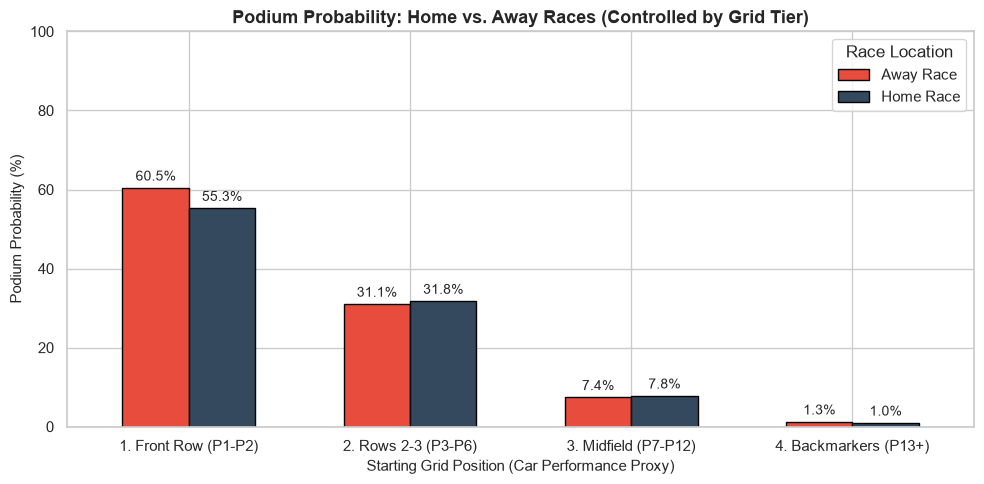
\includegraphics[width=0.85\textwidth]{c38_1.png}
  \caption{Podium probability at home vs.\ away, within grid tiers.}
  \label{fig:q2}
\end{figure}

\subsection{Q3. Which constructors have the highest mechanical-retirement rate in 2014--2021 vs.\ 2022--2024?}
\textbf{Definition and joins.} \ft{results} (deduplicated) $\bowtie$ \ft{races} (year) $\bowtie$ \ft{constructors} (name) $\bowtie$ \ft{status} (our mapping of the 139 statuses). A mechanical retirement is a race start that ended because a car component failed (engine, gearbox, hydraulics, \ldots). Crashes and collisions, driver errors and regulatory outcomes (disqualification) are excluded. The denominator is race starts only: did-not-start and did-not-qualify entries are removed. Constructors need at least 20 starts in both periods (11 teams).

\textbf{Answer.} Figure~\ref{fig:q3}:
\begin{itemize}
  \item \textbf{2014--2021:} highest were \textbf{McLaren (14.5\%)}, \textbf{Sauber (11.0\%)} and \textbf{Red Bull (10.7\%)}.
  \item \textbf{2022--2024:} highest were \textbf{Alfa Romeo (12.5\%)}, \textbf{Alpine (11.0\%)} and \textbf{AlphaTauri (6.8\%)}.
  \item Most teams became much more reliable (McLaren 14.5\%$\to$3.7\%, Red Bull 10.7\%$\to$3.7\%). Alfa Romeo (4.2\%$\to$12.5\%) and Alpine (6.8\%$\to$11.0\%) moved the other way. Mercedes stayed low and stable (4.1\%$\to$4.4\%), and the lowest early-hybrid rate was Aston Martin's (2.3\%).
\end{itemize}

\textbf{Grain, missing data and cutoff.} The grain is one row per car entry per race. Status is a \emph{post-race} outcome: it is used here only to answer the question and is excluded from the modeling table.

\textbf{Caveat.} Teams are grouped by constructor name. Renamed organisations therefore appear as separate teams (Sauber/Alfa Romeo, Toro Rosso/AlphaTauri, Renault/Alpine, Force India/Racing Point/Aston Martin). Some teams fail the 20-starts filter, and the ``2014--2021'' figure for Alpine covers only the 2021 season.

\begin{figure}[!htbp]
  \centering
  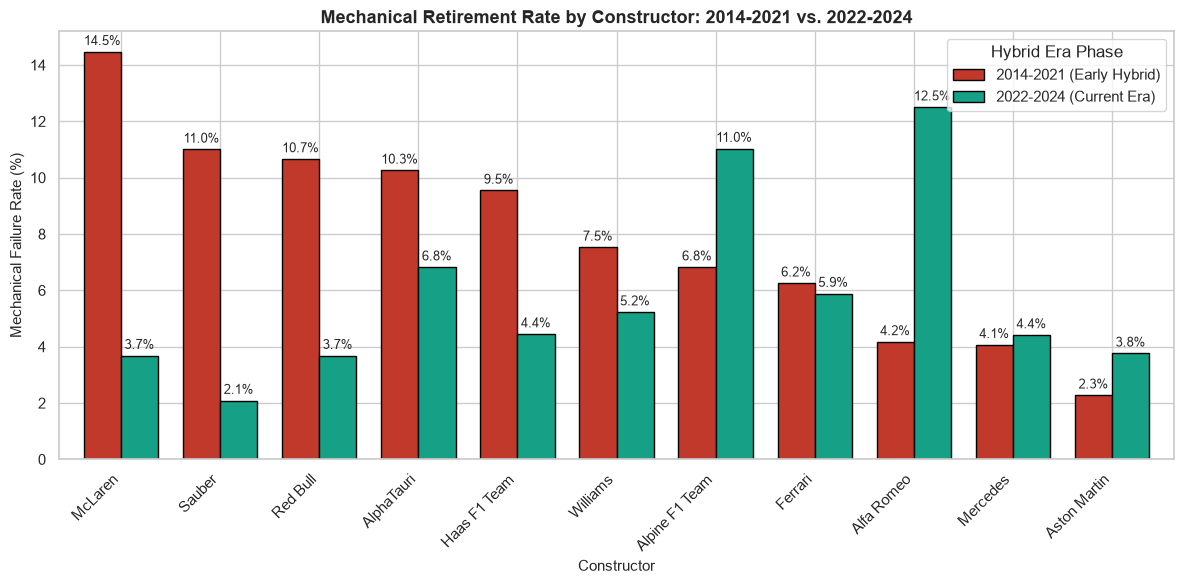
\includegraphics[width=\textwidth]{c42_1.png}
  \caption{Mechanical-retirement rate per constructor, 2014--2021 vs.\ 2022--2024.}
  \label{fig:q3}
\end{figure}

%=====================================================================
\section{Modeling Table and Selected Features}

\subsection{Selected features and why each is valid at the pre-race cutoff}
Table~\ref{tab:features} lists the eight features. Every feature is known once qualifying has finished, before lights out.

\begin{table}[!htbp]
\centering\small
\begin{tabular}{>{\raggedright\arraybackslash}p{4.3cm}>{\raggedright\arraybackslash}p{2.9cm}>{\raggedright\arraybackslash}p{7.2cm}}
\toprule
\textbf{Feature} & \textbf{Source} & \textbf{Why it is valid at the cutoff, and evidence} \\
\midrule
\ft{grid} & \ft{results.grid} & Official starting slot after penalties, fixed before the start. Correlation with podium $r=-0.37$; the largest ablation drop (with pace). Pit-lane starts (\ft{grid}$=0$) are recoded to 20, the back of the grid. \\
\ft{gap\_to\_pole\_pct} & \ft{qualifying} & Single-lap pace relative to pole, from the completed qualifying session. $r=-0.29$. Missing before 1994 and for drivers without a time (61\% of rows overall). \\
\ft{prev\_driver\_points}, \ft{prev\_driver\_wins} & \ft{driver\_standings} & Standings \emph{after the previous race} of the same season (lag of one race within driver--season; 0 at round 1). They never include the current race. $r=0.32$ and $0.37$. \\
\ft{prev\_constructor\_points}, \ft{prev\_constructor\_wins} & \ft{constructor\_\-standings} & Same one-race lag within constructor--season. $r=0.29$ and $0.37$. \\
\ft{driver\_age} & \ft{drivers.dob}, \ft{races.date} & Age on race day, known in advance. $r=0.05$ (kept as a context feature; see ablation). \\
\ft{is\_home\_race} & \ft{drivers}, \ft{circuits} & Nationality vs.\ circuit country, known in advance. $r=-0.02$ (kept to test the Q2 hypothesis inside the model). \\
\bottomrule
\end{tabular}
\caption{Selected features. $r$ = Pearson correlation with \ft{target\_podium} on the full modeling table (Figure~\ref{fig:corr}).}
\label{tab:features}
\end{table}

\textbf{How the form features stay leakage-safe.} The Ergast standings row for race $R$ already includes the result of race $R$. We therefore sort standings by (year, round) and shift by one race inside each driver--season and constructor--season group. The feature attached to race $R$ is then the standing after race $R-1$. Round 1 of each season gets 0, because the championship starts from scratch.

\textbf{Excluded on purpose.}
\begin{itemize}
  \item \ft{position}, \ft{points}, \ft{laps}, \ft{time}, \ft{fastestLap*}, \ft{statusId}, pit stops and lap times: these are post-race and would leak the outcome.
  \item Qualifying position (\ft{quali\_position}): almost the same signal as \ft{grid} (collinear), and missing for most of the history; \ft{grid} is the slot actually used at the start.
\end{itemize}

\begin{figure}[!htbp]
  \centering
  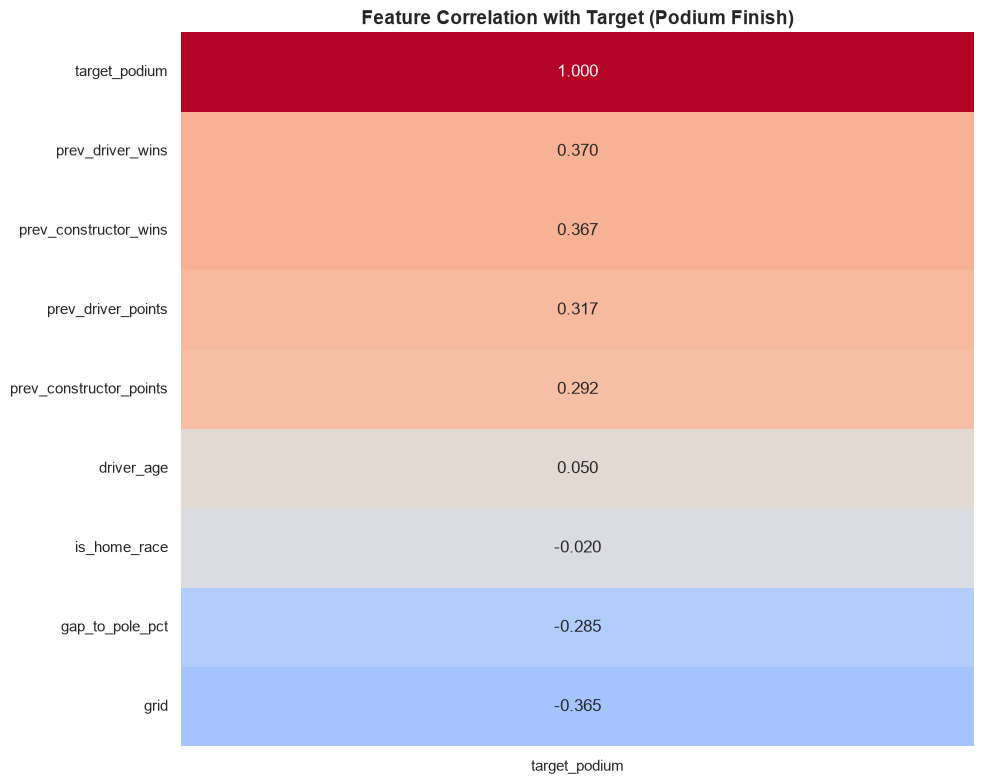
\includegraphics[width=0.55\textwidth]{c45_1.png}
  \caption{Correlation of each selected feature with the podium target.}
  \label{fig:corr}
\end{figure}

\subsection{Preprocessing}
\begin{itemize}
  \item \textbf{Missing pace:} \ft{gap\_to\_pole\_pct} is imputed with a constant 25.0 (a deliberately poor pace) and a binary missing-indicator column is added. The model can therefore tell ``no qualifying time'' apart from a real 25\% gap. The imputer is fitted inside the training pipeline only.
  \item \textbf{Scaling:} \ft{StandardScaler} for logistic regression and the neural network, fitted on training data only. The random forest uses unscaled inputs.
  \item \textbf{Class imbalance:} 12.7\% positives. We use \ft{class\_weight='balanced'} for logistic regression and the random forest, and balanced class weights for the neural network.
\end{itemize}

\subsection{Chronological split}
\begin{itemize}
  \item \textbf{Train:} 1950--2018 (24,109 rows).
  \item \textbf{Validation:} 2019--2021 (1,200 rows).
  \item \textbf{Test:} 2022--2024 (1,359 rows, never used for any choice).
\end{itemize}
A random split would let the model learn from races \emph{after} the ones it is tested on, and would mix seasons whose standings features are linked across rounds. A time-ordered split mimics real use (predict the next seasons from the past). The test period starts with the 2022 ground-effect regulations, so it is also a test of generalisation to a new era.

%=====================================================================
\section{Models and Results}

\subsection{Models}
\begin{itemize}
  \item \textbf{Baseline: logistic regression} (L2-regularised, balanced class weights). A linear model of the log-odds; simple, stable and interpretable. Its limitation is that it cannot represent thresholds or interactions.
  \item \textbf{Random forest} (200 trees, \ft{max\_depth}=7, balanced class weights). An ensemble of decision trees that captures non-linear effects and interactions, e.g.\ ``front row \emph{and} strong team''. The depth limit controls overfitting. Its limitations: probabilities are less smooth, and it splits credit among correlated features.
  \item \textbf{Shallow neural network} (Keras: 32 ReLU $\to$ dropout 0.2 $\to$ 16 ReLU $\to$ sigmoid; Adam, binary cross-entropy, 100 epochs, batch 64, balanced class weights). It learns smooth non-linear functions. Its limitations: it needs scaled inputs, is the least interpretable, and its results vary slightly between training runs.
\end{itemize}

\subsection{Metric choice}
\begin{itemize}
  \item \textbf{Primary metric: PR-AUC.} Podiums are only 12.7\% of rows, and the task is to rank the few true podium finishers above everyone else. PR-AUC focuses on that positive class and, unlike ROC-AUC, is not inflated by the many easy negatives (a random model scores about 0.13).
  \item \textbf{Secondary metric: F1} at the 0.5 probability threshold. It measures the precision--recall trade-off of an actual podium yes/no prediction.
  \item ROC-AUC, precision and recall are also reported.
\end{itemize}

\subsection{Model comparison}
\begin{table}[!htbp]
\centering\small
\setlength{\tabcolsep}{4pt}
\begin{tabular}{lccccc|ccccc}
\toprule
& \multicolumn{5}{c|}{\textbf{Validation (2019--2021)}} & \multicolumn{5}{c}{\textbf{Test (2022--2024)}}\\
\textbf{Model} & ROC & \textbf{PR} & F1 & Prec. & Rec. & ROC & \textbf{PR} & F1 & Prec. & Rec.\\
\midrule
Logistic regression (baseline) & 0.925 & 0.707 & 0.590 & 0.436 & 0.911 & 0.923 & 0.646 & 0.571 & 0.408 & 0.951\\
Random forest & 0.934 & 0.721 & 0.612 & 0.461 & 0.911 & \textbf{0.928} & \textbf{0.667} & 0.608 & 0.451 & 0.931\\
Shallow neural network & 0.934 & \textbf{0.746} & \textbf{0.657} & 0.523 & 0.883 & 0.925 & 0.651 & \textbf{0.641} & 0.501 & 0.887\\
\bottomrule
\end{tabular}
\caption{All five metrics on validation and on the unseen test set (full-history training). Training-set scores: LR ROC/PR/F1 = 0.897/0.545/0.514; RF = 0.916/0.619/0.546.}
\label{tab:models}
\end{table}

\textbf{Interpretation.}
\begin{itemize}
  \item All models generalise well. LR and RF even score lower on the (older, harder) training seasons than on the test seasons, so there is no sign of overfitting to 1950--2018.
  \item The \textbf{random forest} earns its extra complexity on the primary metric: test PR-AUC 0.667 vs.\ 0.646 for the baseline.
  \item The \textbf{neural network} is best on validation PR-AUC and on test F1 (0.641), because it trades some recall for clearly higher precision.
  \item The baseline has the highest recall (0.951) but the lowest precision. At the 0.5 threshold with balanced weights it predicts too many podiums.
  \item The gap between models is small compared with how much each depends on \ft{grid} (Section~\ref{sec:ablation}). Most of the signal is captured even by a linear model.
\end{itemize}

\begin{figure}[!htbp]
  \centering
  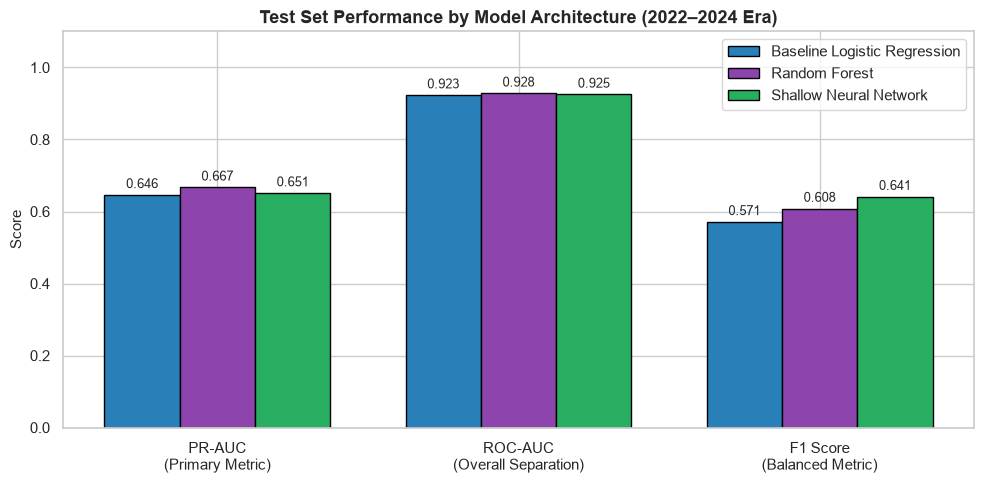
\includegraphics[width=0.8\textwidth]{c60_1.png}
  \caption{Test-set (2022--2024) performance of the three models.}
\end{figure}

\subsection{Additional modeling attempt: era-restricted training (2006+)}
As a further attempt, all three models were retrained on 2006--2018 only (5,355 rows, the knockout-qualifying era, with almost no imputation) and evaluated on the same validation and test sets (Figure~\ref{fig:era}). Results on the test set:
\begin{itemize}
  \item \textbf{Logistic regression:} PR-AUC 0.653 (vs.\ 0.646 on full history), F1 0.612 (vs.\ 0.571).
  \item \textbf{Neural network:} PR-AUC 0.676, the best value of either setting.
  \item \textbf{Random forest:} PR-AUC 0.650 (vs.\ 0.667), so less data hurt it here.
\end{itemize}
Training only on the modern era therefore helps the linear and neural models but not the forest. This is evidence of era sensitivity: older seasons add data but also distribution shift.

\begin{figure}[!htbp]
  \centering
  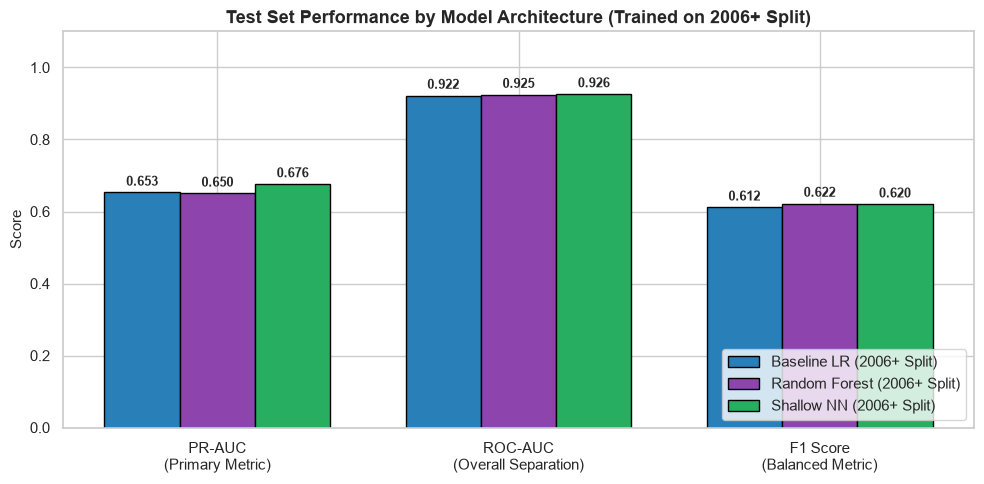
\includegraphics[width=0.75\textwidth]{c65_1.png}
  \caption{Test-set performance when training on 2006--2018 only.}
  \label{fig:era}
\end{figure}

%=====================================================================
\section{Feature-Group Ablation}\label{sec:ablation}
Each feature group was removed in turn and the random forest was retrained (Table~\ref{tab:abl}, Figure~\ref{fig:abl}).

\begin{table}[!htbp]
\centering\small
\begin{tabular}{llcc}
\toprule
\textbf{Group removed} & \textbf{Features} & \textbf{Test PR-AUC} & \textbf{Drop}\\
\midrule
None (full model) & -- & 0.667 & -- \\
Track position \& pace & \ft{grid}, \ft{gap\_to\_pole\_pct} & 0.466 & \textbf{+0.200}\\
Historical form & 4 lagged standings features & 0.638 & +0.028\\
Driver context & \ft{driver\_age}, \ft{is\_home\_race} & 0.673 & $-0.006$\\
\bottomrule
\end{tabular}
\caption{Feature-group ablation (random forest, test PR-AUC).}
\label{tab:abl}
\end{table}

\begin{itemize}
  \item \textbf{Track position and pace} carry most of the signal.
  \item \textbf{Championship form} adds a smaller but real gain: it separates strong teams that start out of position from weak teams that qualified well.
  \item \textbf{Driver context} adds nothing (removing it slightly improves PR-AUC). This is consistent with Q2 and with its near-zero correlations.
\end{itemize}

\begin{figure}[!htbp]
  \centering
  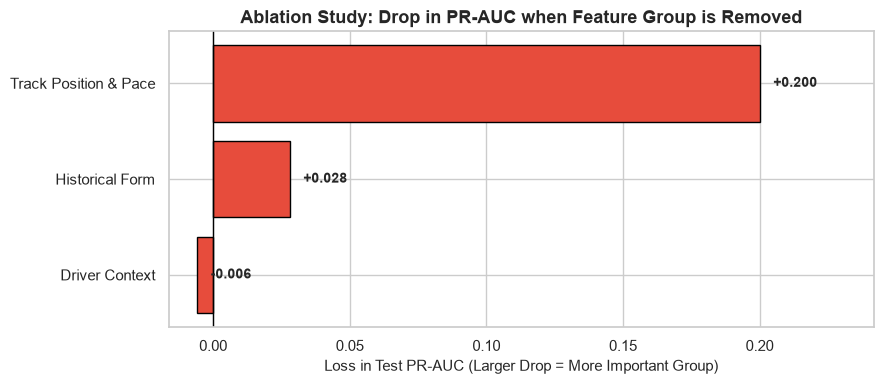
\includegraphics[width=0.7\textwidth]{c69_1.png}
  \caption{Drop in test PR-AUC when each feature group is removed.}
  \label{fig:abl}
\end{figure}

%=====================================================================
\section{Model Explainability (XAI)}
All three models are explained on the unseen 2022--2024 test set. SHAP and LIME use the full 1950--2018 training set (after the pipeline's own imputer) as their reference, and SHAP values are reported in \textbf{percentage points of P(podium)}. These explanations show what the models \emph{rely on} to predict, not what \emph{causes} a podium finish.

\subsection{Global: permutation importance}
Each test feature was shuffled 30 times (the same shuffles for every model) and the drop in PR-AUC was recorded (Figure~\ref{fig:perm}).
\begin{itemize}
  \item \ft{grid} gives the largest, statistically reliable drop for every model (0.29 LR, 0.34 RF, about 0.4 NN).
  \item Form features follow, but each model leans on different ones: LR on driver points, the NN on driver points and wins, the RF on win counts. The standings features are strongly correlated ($\rho=0.96$ between driver and constructor points), so they can stand in for each other.
  \item \ft{gap\_to\_pole\_pct}, \ft{driver\_age} and \ft{is\_home\_race} have almost no effect; pace is largely redundant with \ft{grid} ($\rho=0.82$).
\end{itemize}

\begin{figure}[!htbp]
  \centering
  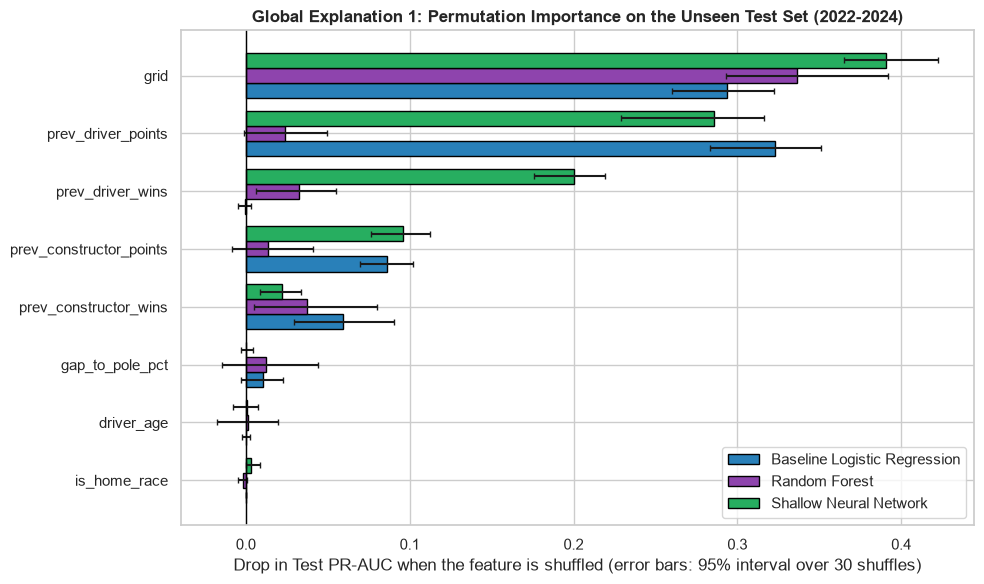
\includegraphics[width=0.78\textwidth]{c75_1.png}
  \caption{Permutation importance: drop in test PR-AUC (95\% interval over 30 shuffles).}
  \label{fig:perm}
\end{figure}

\subsection{Global: SHAP}
\begin{itemize}
  \item \ft{grid} is the top SHAP feature for all three models (Figure~\ref{fig:bee}). A front-row start adds roughly 30--50 points to P(podium); a start at the back removes about 20.
  \item The dependence plots (Figure~\ref{fig:dep}) show different shapes for the grid effect. LR declines smoothly. The RF learned a step: a flat bonus for P1--P4, a steep drop through P5--P9 and little change behind P10. The NN learned a smooth version of that step.
  \item High \ft{prev\_constructor\_points} pushes LR and NN predictions \emph{down}. This is a collinearity effect, not a team effect: once driver points are known, constructor points mostly add the teammate's points.
  \item Permutation and SHAP rankings agree strongly for LR (Spearman $\rho=0.93$) and moderately for RF and NN ($\rho\approx0.64$).
\end{itemize}

\begin{figure}[!htbp]
  \centering
  \begin{subfigure}{0.325\textwidth}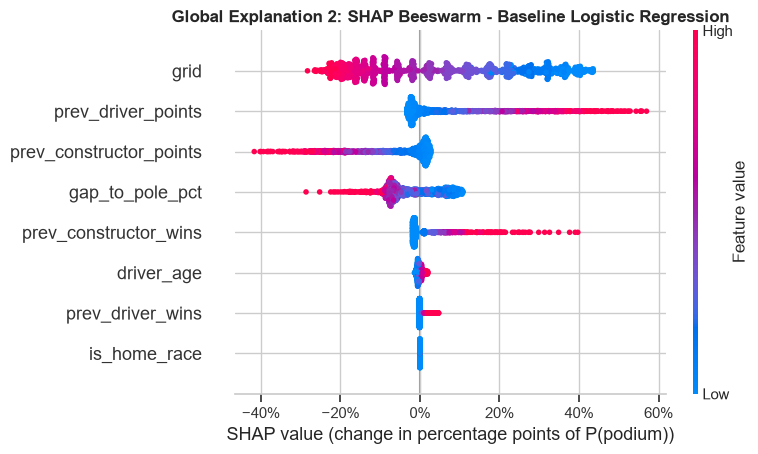
\includegraphics[width=\textwidth]{c78_1.png}\caption{Logistic regression}\end{subfigure}
  \begin{subfigure}{0.325\textwidth}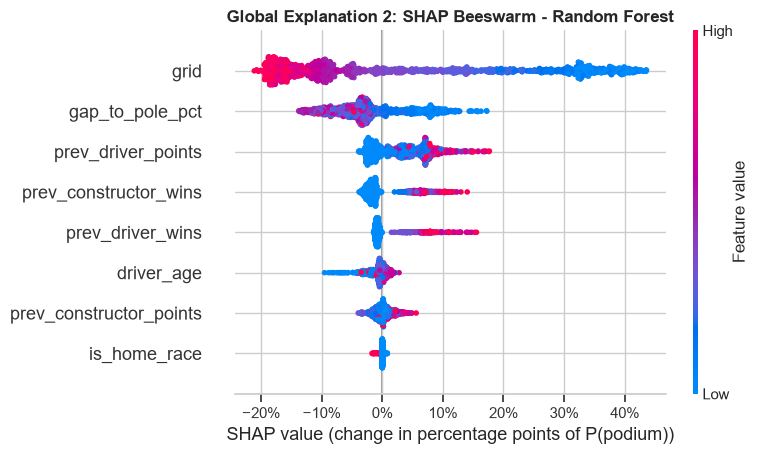
\includegraphics[width=\textwidth]{c78_2.png}\caption{Random forest}\end{subfigure}
  \begin{subfigure}{0.325\textwidth}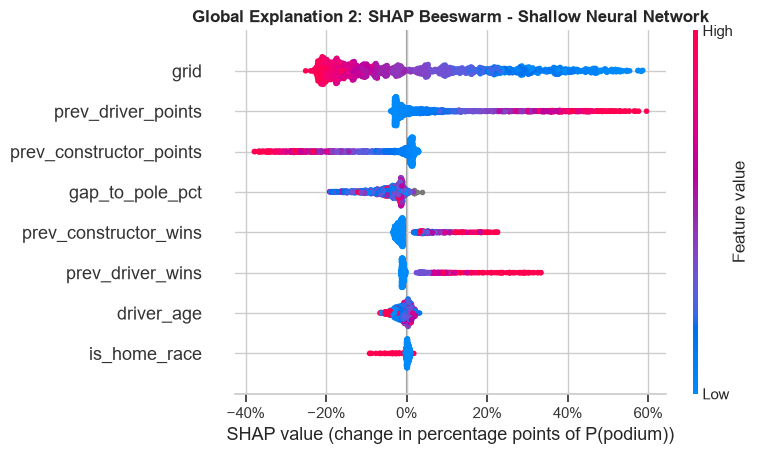
\includegraphics[width=\textwidth]{c78_3.png}\caption{Neural network}\end{subfigure}
  \caption{SHAP beeswarm plots (percentage points of P(podium)). Each dot is one test row; colour is the feature value.}
  \label{fig:bee}
\end{figure}

\begin{figure}[!htbp]
  \centering
  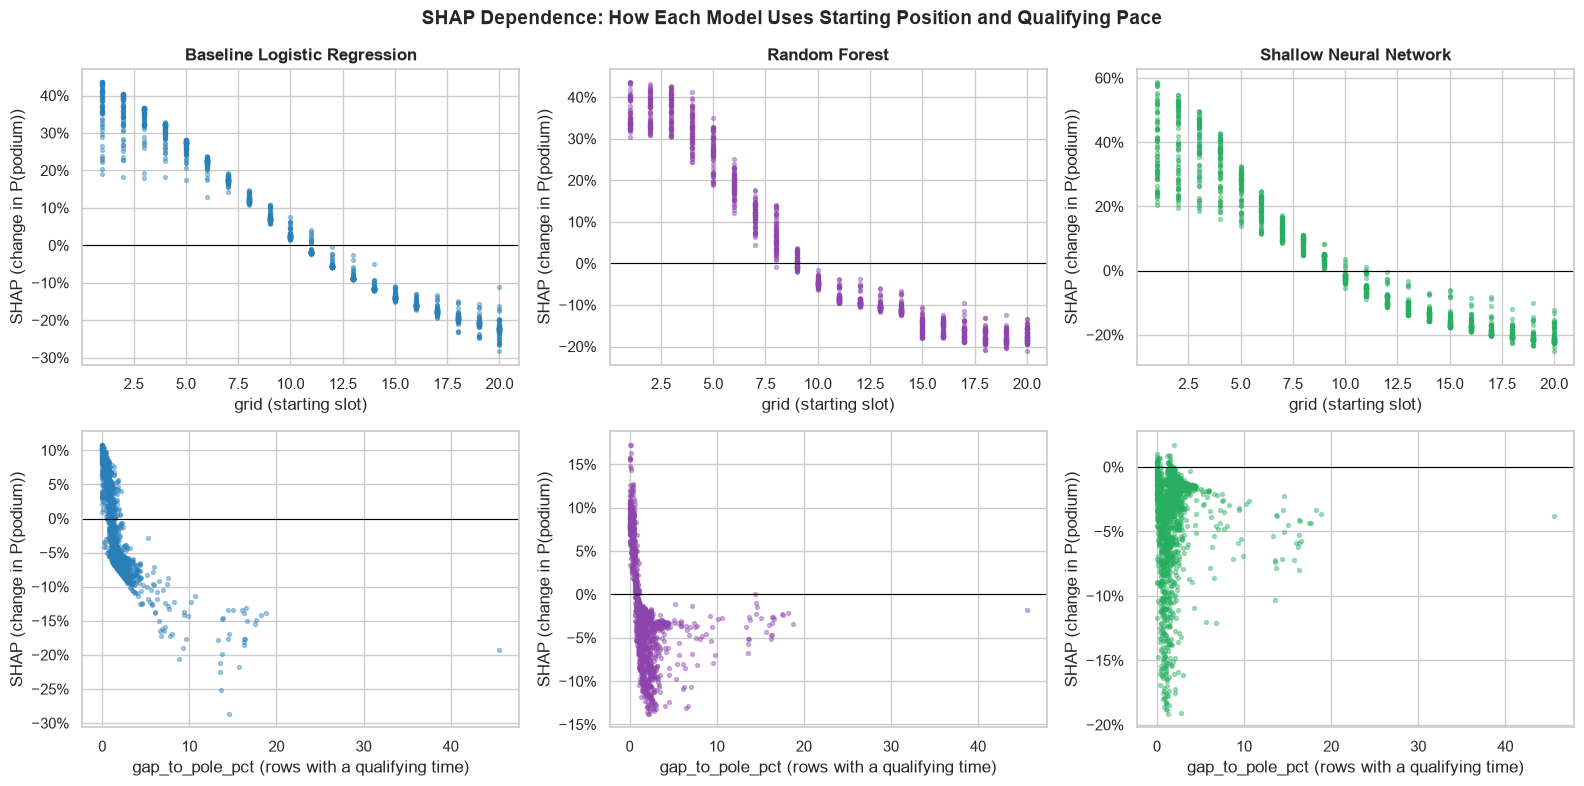
\includegraphics[width=0.92\textwidth]{c79_2.png}
  \caption{SHAP dependence of \ft{grid} (top) and \ft{gap\_to\_pole\_pct} (bottom).}
  \label{fig:dep}
\end{figure}

\subsection{Local: SHAP waterfalls and LIME}
Two real test rows were explained:
\begin{itemize}
  \item \textbf{Record A, complete:} Max Verstappen, 2024 São Paulo GP. He started P17 and won.
  \item \textbf{Record B, partially missing:} Sergio Pérez, 2023 Australian GP. He had no qualifying time, started 20th and finished P5.
\end{itemize}

\textbf{Record A.} All three models predicted a podium (P = 0.62 LR, 0.74 RF, 0.77 NN). \ft{grid}$=17$ lowers every prediction, but his championship form (362 points, 7 wins) outweighs it (e.g.\ +57 points from driver points in LR).

\textbf{Record B.} The models disagree (0.06 LR vs.\ 0.42 RF and 0.34 NN). \ft{grid}$=20$ is the main negative in all three. The missing qualifying time has only a small net effect, because the imputed value and the missing flag largely cancel.

\begin{figure}[!htbp]
  \centering
  \begin{subfigure}{0.325\textwidth}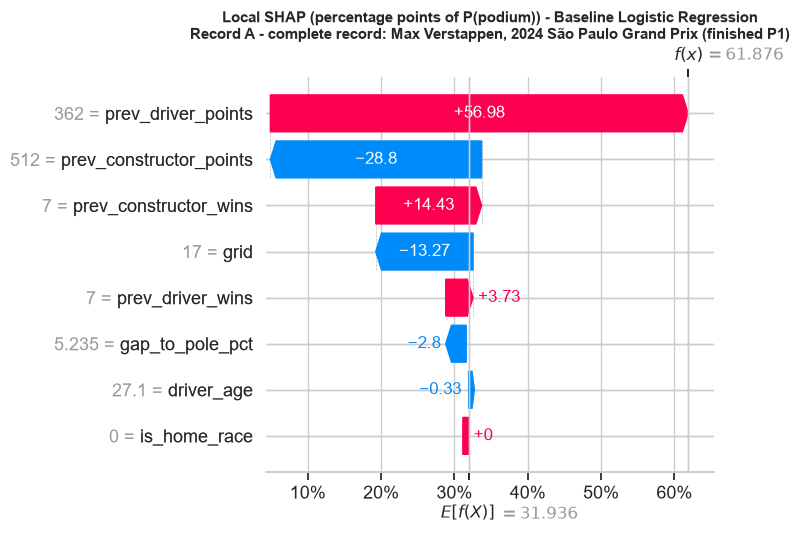
\includegraphics[width=\textwidth]{c83_1.png}\end{subfigure}
  \begin{subfigure}{0.325\textwidth}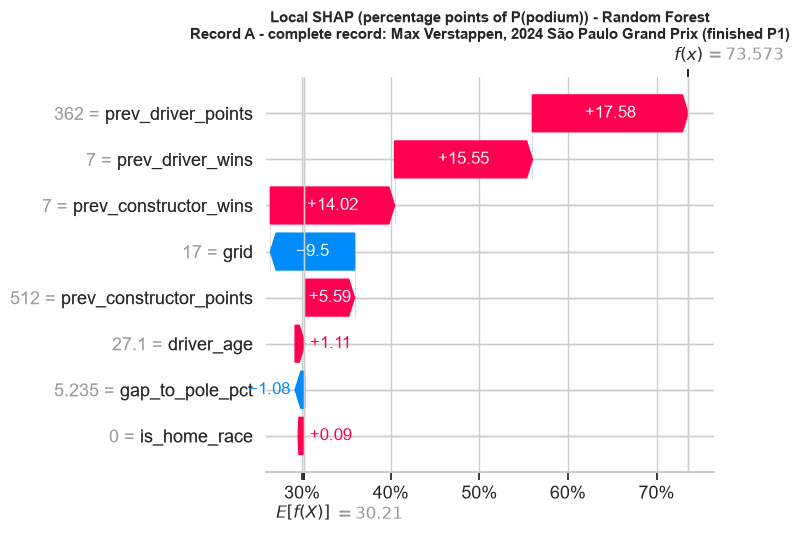
\includegraphics[width=\textwidth]{c83_2.png}\end{subfigure}
  \begin{subfigure}{0.325\textwidth}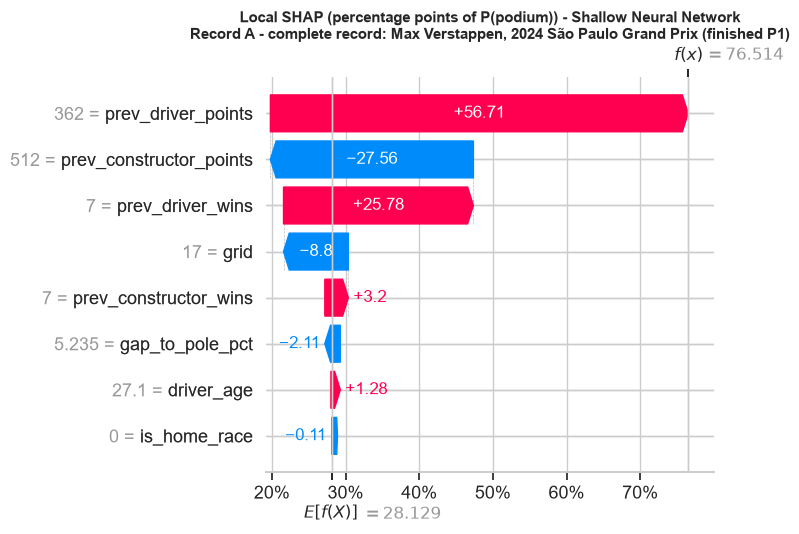
\includegraphics[width=\textwidth]{c83_3.png}\end{subfigure}\\[4pt]
  \begin{subfigure}{0.325\textwidth}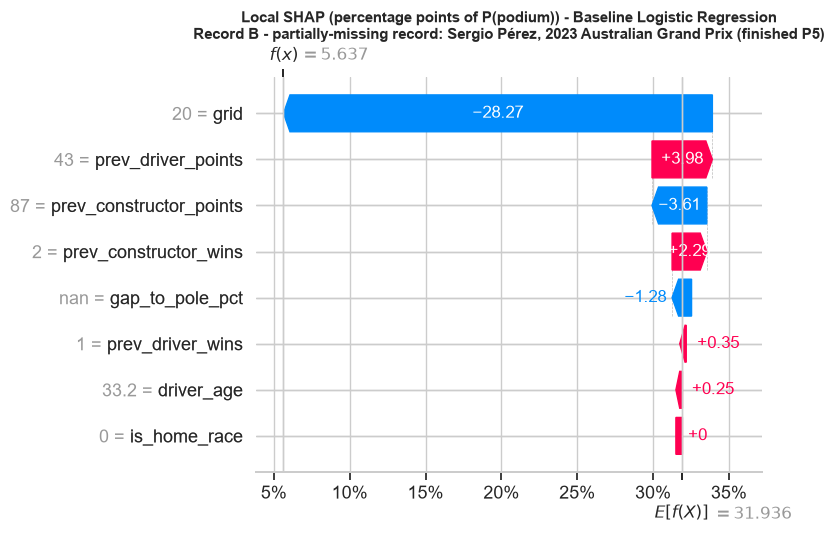
\includegraphics[width=\textwidth]{c83_4.png}\end{subfigure}
  \begin{subfigure}{0.325\textwidth}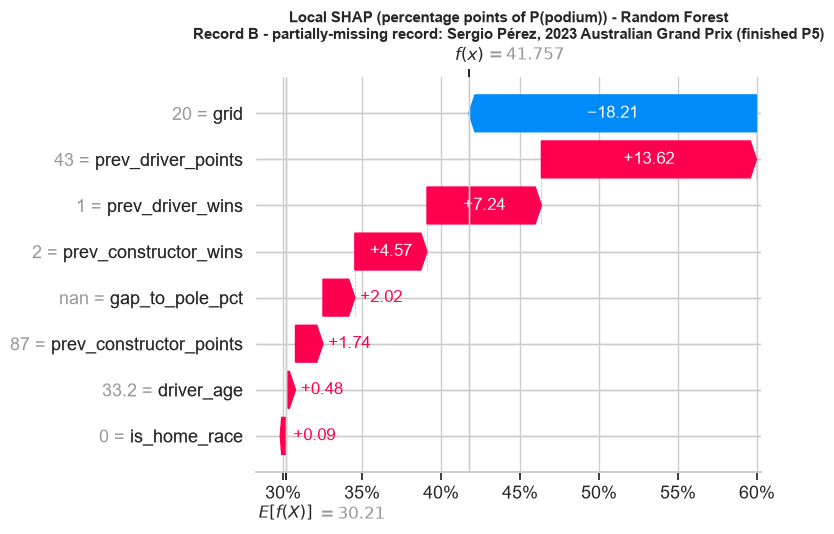
\includegraphics[width=\textwidth]{c83_5.png}\end{subfigure}
  \begin{subfigure}{0.325\textwidth}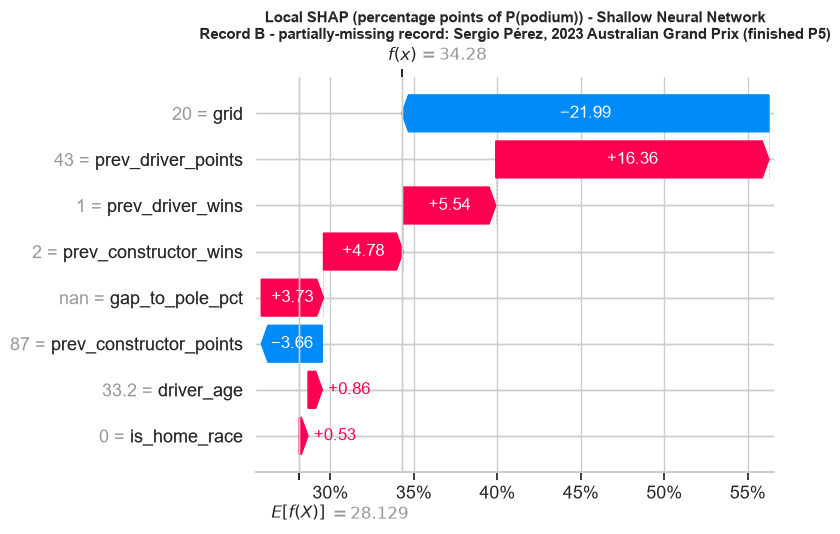
\includegraphics[width=\textwidth]{c83_6.png}\end{subfigure}
  \caption{Local SHAP waterfalls (percentage points of P(podium)). Top: record A. Bottom: record B. Columns: LR, RF, NN.}
  \label{fig:wf}
\end{figure}

\textbf{LIME} gives the same direction as SHAP: the back-of-grid rule is the main negative and form is the main positive (Figure~\ref{fig:lime}). Its local fit is only moderate ($R^2\approx0.25$--$0.65$), so SHAP is used as the primary local explanation.

\begin{figure}[!htbp]
  \centering
  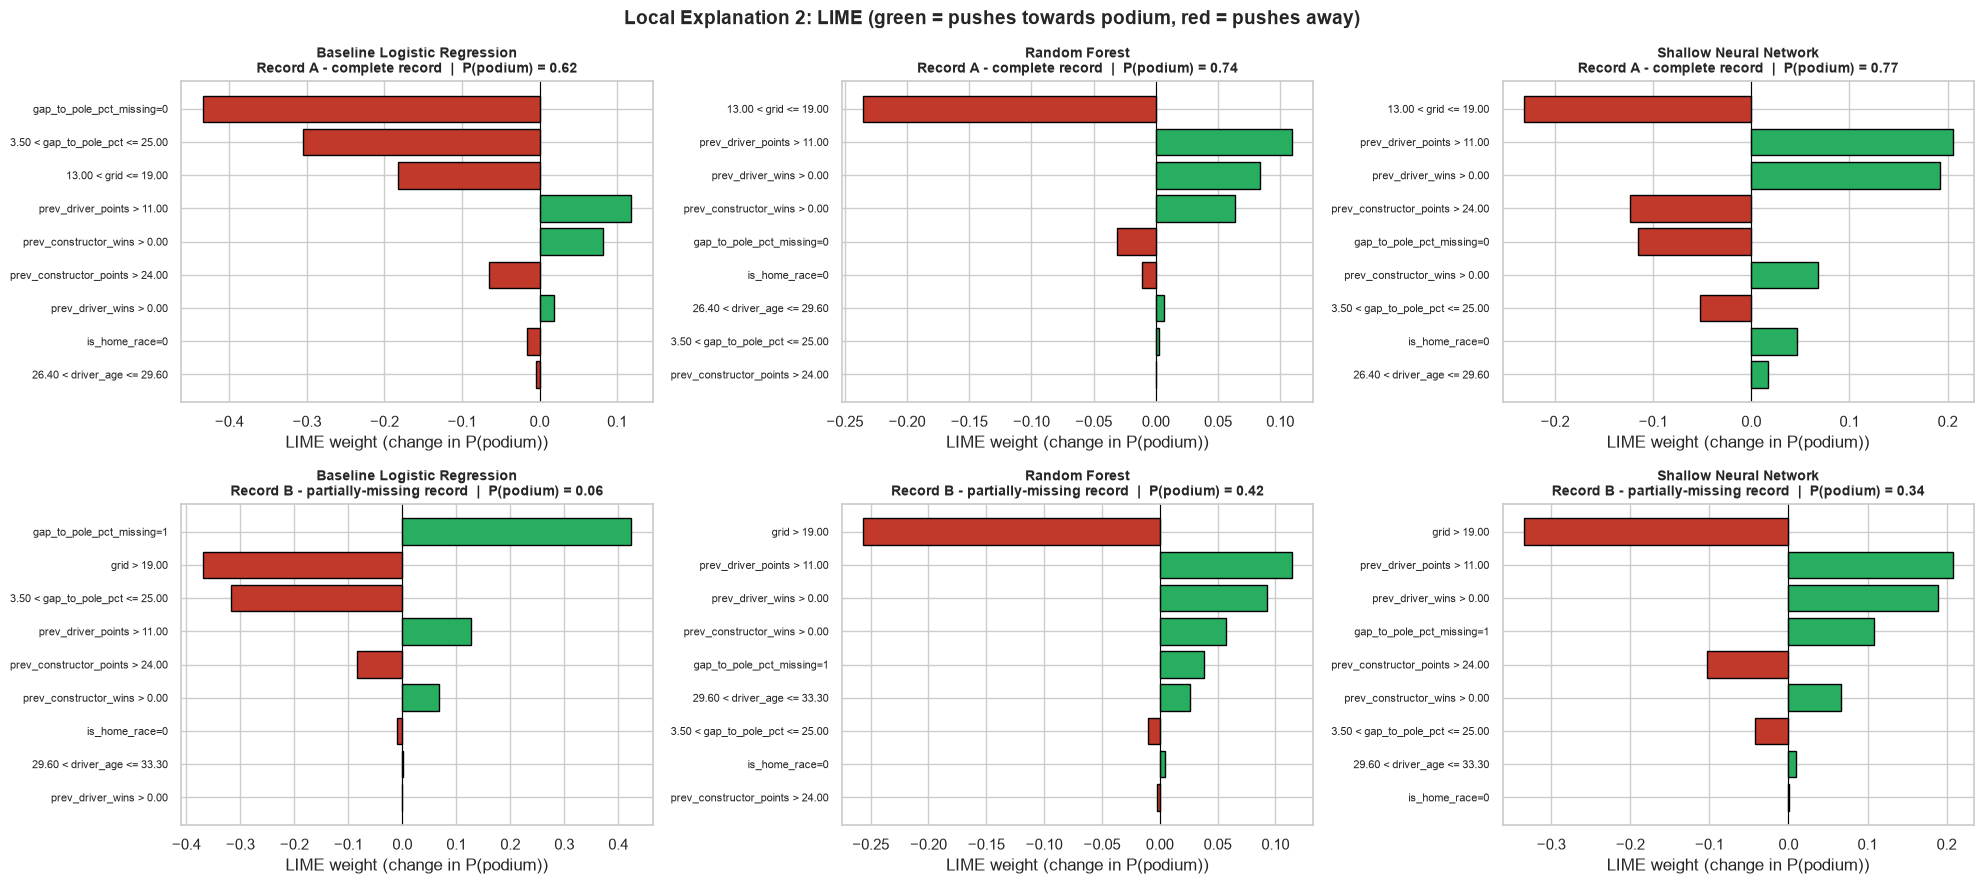
\includegraphics[width=\textwidth]{c86_1.png}
  \caption{LIME explanations for records A (top) and B (bottom).}
  \label{fig:lime}
\end{figure}

%=====================================================================
\section{Known Limitations}
\begin{itemize}
  \item \textbf{Historical qualifying-coverage drift.} The qualifying table only starts in 1994, and its format changed (single session until 2005, knockout from 2006). \ft{gap\_to\_pole\_pct} is missing for 61\% of all rows and 68\% of training rows, but only 1\% of test rows. The imputation and missing flag let us keep the history, but the flag partly encodes ``old era'' rather than ``slow car''.
  \item \textbf{Era sensitivity.} Points systems changed several times (e.g.\ 2003 and 2010), so the scale of the lagged points features is not comparable across decades. Car reliability, grid sizes and overtaking difficulty also changed. The era-restricted experiment shows model rankings shift with the training window, and the 2019--2021 validation seasons were unusually predictable.
  \item \textbf{Small evaluation sets.} Validation and test have 1,200 and 1,359 rows (about 150--200 podiums each). Differences of about 0.01--0.02 in PR-AUC between models are within sampling noise.
  \item \textbf{Fixed threshold.} F1, precision and recall are computed at the default 0.5 threshold with balanced class weights. The threshold was not tuned on validation, which explains the high recall but low precision of the baseline.
  \item \textbf{Form features.} Standings are lagged by one race and reset at round 1, so early-season rows carry little form information. Rows without a standings entry are filled with 0.
  \item \textbf{Neural-network variability.} Retraining the network gives slightly different scores (test PR-AUC about 0.65--0.68 across our runs), so its ranking against the random forest is not stable.
  \item \textbf{Data-engineering questions.} Grands Prix and constructors are grouped by name, so renamed teams and changed circuit layouts are split or merged. Hybrid-era circuit rates rest on few starts.
  \item \textbf{Explanations.} SHAP and LIME depend on the chosen reference population, and correlated features make single-feature attributions unstable. None of the explanations are causal.
\end{itemize}

\end{document}
